\chapter{Implementation}
\label{chap:implementation}

\ifpdf
    \graphicspath{{Chapter3/Chapter3Figs/PDF/}{Chapter3/Chapter3Figs/PNG/}
		{Chapter3/Chapter3Figs/}}
\else
    \graphicspath{{Chapter3/Chapter3Figs/EPS/}{Chapter3/Chapter3Figs/}}
\fi

This chapter discusses the implementation issues in more detail.  It also
explains the filesystem interface and how it can be used.  We will show how
the filesystem interface and independence of nodes gives much desired
flexibility.  We will see some examples showing how easy it is to run
applications on this platform. This chapter concentrates on how XCPU3 was
implemented and describes implementation decisions which have proven to be
important.


\section{Inferno}
Before we start discussing our decision to use Inferno, let us explain what
Inferno is.  Inferno\cite{inferno} is an open source distributed operating
system developed and maintained by \textit{Vita Nuova}.  It is a  direct descendant
of the \textbf{Plan 9} operating system.  It runs natively on multiple
hardware platforms and can also run as a user-space application on top of other
operating systems.  For the purpose of this project \textit{"hosted Inferno OS"} or
\textit{"userspace Inferno"} refers to Inferno running as user-space
application on top of other operating systems. So we will use these terms
interchangeably.

As we are aiming for a flexible heterogeneous environment with different
operating systems and different architectures, we found the Inferno operating
system to be an attractive platform.  It allowed us to develop XCPU3 once and
easily deploy it on different platforms while enjoying the Plan 9 features
on all those platforms.

This decision does come with the cost of some performance loss.  Each node needs
to run hosted Inferno in user-space which takes up some resources of the node. 
Also every communication with the filesystem involves invocation of the host
kernel which then passes the call to the guest inferno. The responses
follow the same path.  This does add latency in communication leading to
poorer performance compared to filesystems implemented natively on host
operating systems. But we are willing to accept this performance loss for achieving 
the portability to a large number of platforms.

We also had a choice of developing XCPU3 as part of the Inferno kernel or as an Inferno user-space
application.  User-space development is comparatively easy and user-space tools
can be used for debugging any problems.  On the other hand, kernel-space development
comes with more constraints and practically no support for debugging.  Any bug
in kernel-space code typically leads to a kernel panic giving very little information
about the cause of the bug.  The advantage of kernel-space development is that serving
user requests coming to XCPU3 will not involve context switches between Inferno
user-space and kernel-space.  As the choice between Inferno kernel-space and user-space
does not affect the portability, we decided to implement XCPU3 in Inferno kernel-space
for better performance.  We are also hoping that this decision will help in
easily developing a high performance native Plan 9 port for XCPU3 as the code-base of
Plan 9 and Inferno kernel are similar.


Our choice of Inferno gave us the flexibility and features of the Plan 9 operating
system on other operating systems.  It allowed us to quickly implement and
deploy our filesystem on multiple platforms easily at the cost of some
performance.


\section{Implementation}

XCPU3 is implemented as the filesystem in the Inferno kernel.  Figure 
\ref{fig:XCPU3} shows the placement of XCPU3 in the context of applications, host 
operating system and the Inferno.

\begin{figure}[h]
  \begin{center}
    \leavevmode
    \ifpdf
      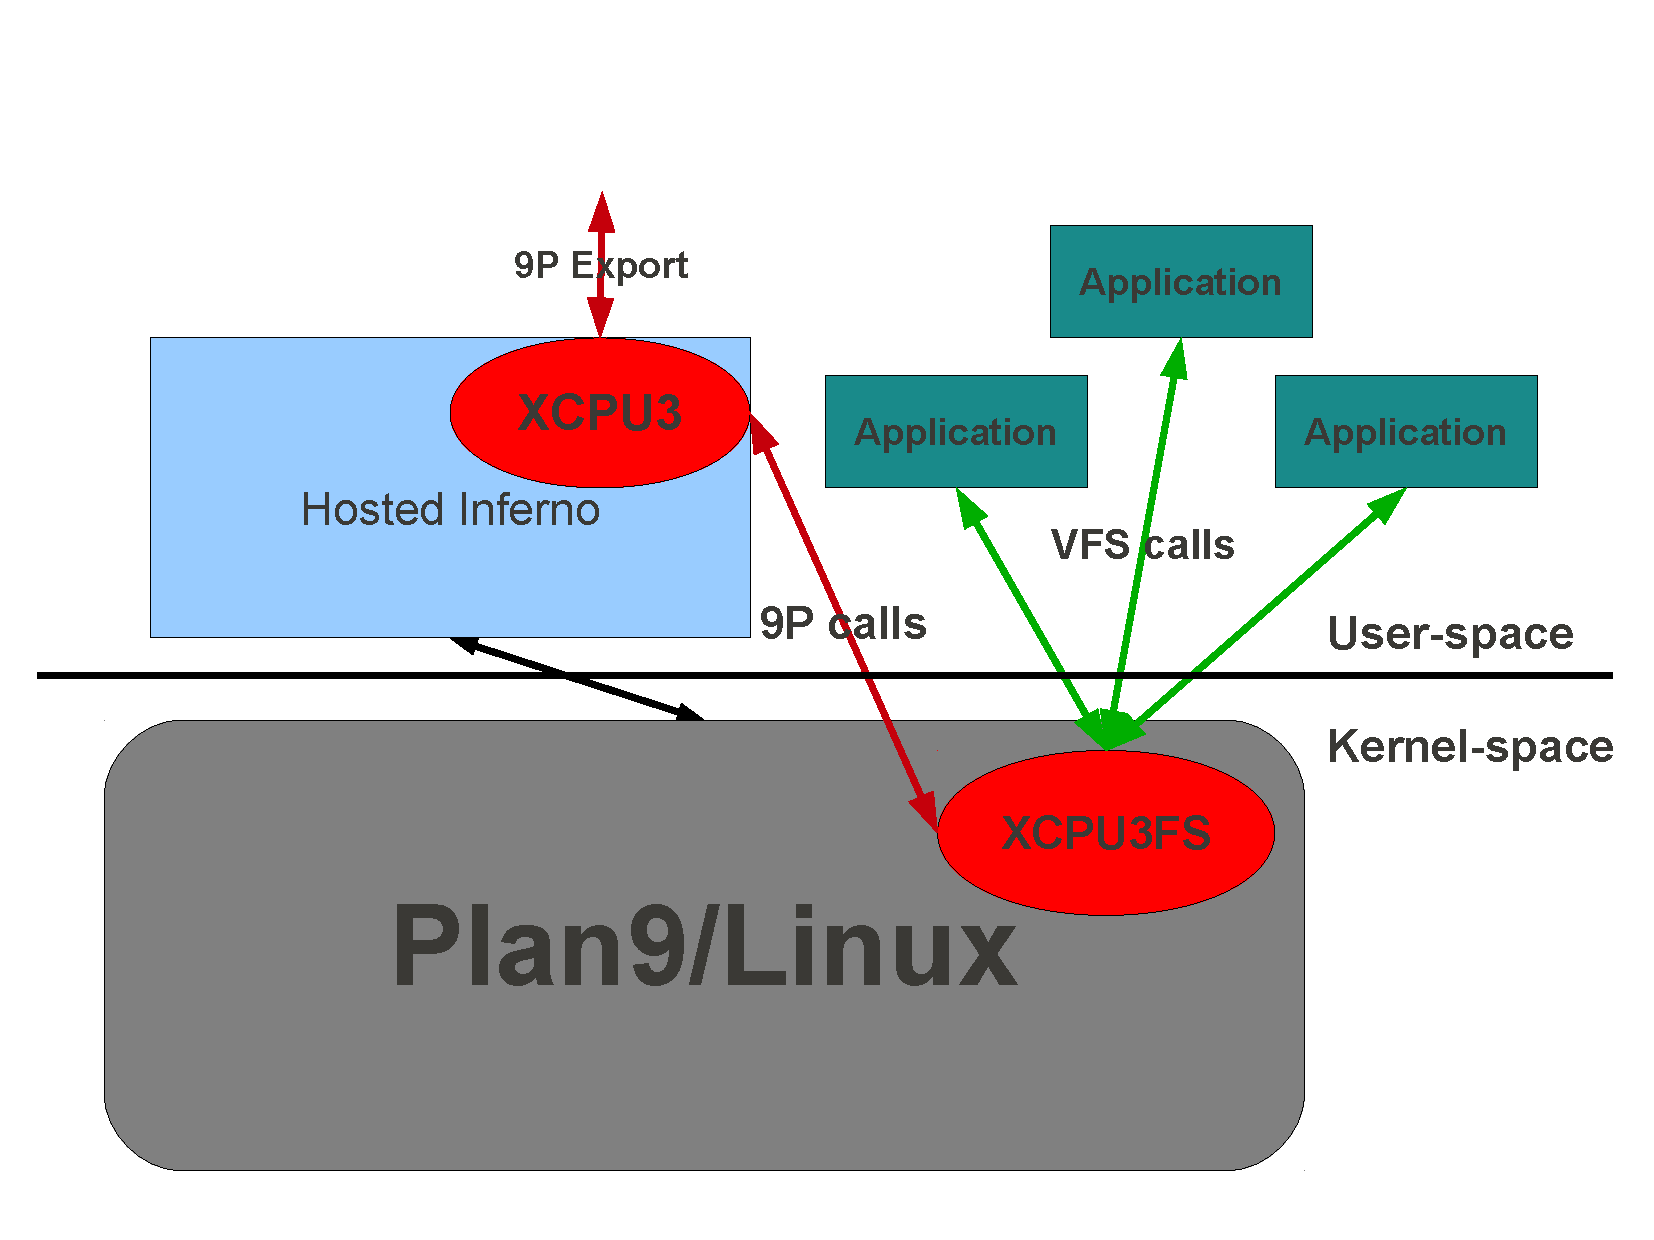
\includegraphics[height=0.4\textheight,width=0.6\textwidth]
		{XCPU3Structure}
    \fi
    \caption{XCPU3 Structure}
    \label{fig:XCPU3}
  \end{center}
\end{figure}

The XCPU3 filesystem is exported by Inferno using the \texttt{9P} protocol.  This protocol
is used by Plan 9 and Inferno extensively to access any file.  Recently the Linux kernel
has added support for the \texttt{9P} protocol\cite{graverobbers}.  This allows Linux to mount filesystems
exported over the 9P protocol.  Other Unix based operating systems can use FUSE\cite{FUSE} 
for accessing the 9P based filesystems.  As FUSE based filesystems run in user-space, 
they perform slower compared to native filesystems implemented in the kernel.  
But implementing FUSE based filesystems is much easier and faster.  Applications
can directly use the FUSE based filesystem just like a kernel implemented filesystem with the same API. 
Applications can also directly talk with filesystems exported over \texttt{9P} by implementing
the client side of the \texttt{9P} protocol.  This way they can get better performance
by bypassing VFS and/or FUSE interfaces.


In a typical setup, Inferno runs in the hosted environment on an operating system like Linux
or Plan 9.  On its startup this hosted inferno will export the XCPU3 filesystem.
This exported filesystem is mounted by the local host operating system.  
The applications interact with this mounted XCPU3 filesystem using the native interface.
Any interaction with this XCPU3 filesystem is communicated to Inferno using 9P.
The XCPU3 kernel module inside the inferno kernel then receives and interprets the 
user actions.  If needed, it uses services from the host operating system or from
other XCPU3 filesystems deployed on remote locations. The XCPU3 filesystem then 
sends the prepared response over 9P. The host operating system will relay this
response back to the application via the local filesystem interface.


As we discussed before in the Design chapter this XCPU3 is an independent unit, providing
the functionality of reservation, job management and computation.  In the case of an
isolated instantiation, any reservation request is satisfied using local resources.
This way, the application can use the same semantics for both local and remote executions.

\section{The big picture (connecting multiple XCPU3 nodes)}
The real power of the XCPU3 is the ability to connect with each other and form bigger
instance of XCPU3.  XCPU3 filesystem uses the \texttt{9P} protocol to connect with each
other.  This protocol provides access to both local and remote filesystems in 
the same way.  This allows every node to access the XCPU3 filesystem hosted on any node
without worrying about complexities of accessing remote filesystems.  Those
complexities are handled by the \texttt{9P} protocol.


\subsection{Central Services}

The ability to configure many XCPU3 nodes into hierarchy is provided by the
\textit{central services}.  In contrary to the name, central services is
highly distributed and every XCPU3 runs an independent instance of the central
services.  The administrator or the user of each XCPU3 instance need to
provide only the information about its parent and children in the hierarchy and
the all XCPU3 nodes initiate these connections leading to the distributed
creation of the XCPU3 node hierarchy.


Central services is aimed to make all the resources addressable in the
network-oblivious fashion.  It also aims to have external entities
(such as end-user workstations) participate in the hierarchy.  It is also aimed
to be able to work through multiple networks, NAT gateways and firewalls. 
Overall, central services is aimed to grants us a flexible facility for
building hierarchies across different types of network and network
boundaries in a distributed and secure fashion.

\subsubsection{Implementation}
The central services synthetic file server itself is quite
simple.  It provides a simple hierarchy of directory mount points
representing remote nodes.  Mounts of the remote nodes or binds of
previously mounted remote nodes are accomplished within this file
system such that anyone who mounts our name space can also see (and
access) anyone we have mounted transitively,  in such a way a child
node can access a parent nodes, other children, or the parents nodes
parent and so forth.


The original implementation of the central services mechanism used an
auto-mounter-like interface.  When you referenced a name within the
synthetic file server for the first time, it would establish a
connection to that systems central-services server and establish a
“duct”.  A duct is essentially a two way pipeline that allows the
client to mount the sever and vice-versa -- allowing each side to
access the others resources.   Each would create an entry in their
respective mount table based on the node-name.  This allowed clients
sitting behind network-address-translation gateways to contact a
parent and the parent to access that child without having to
re-traverse the gateway.  A command-line option could be used when
starting central services allowing it to connect to a single remote
resource over an ssh-connection establishing a tunnel capable of
crossing firewalls.


It proved difficult to debug and did not allow us to leverage
previously mounted filesystem (such as the parent's root filesystem
from which we get our root filesystem).  A second lighter weight
version of the filesystem was created which allowed manipulation of
the name space via a single control file at the top level with a
simple name space oriented syntax:

\begin{itemize}
	\item Establish a network connection and mount table.
\begin{verbatim}
mount <remote-address> <name>
\end{verbatim}

	\item Bind previously mounted resources.
\begin{verbatim}
bind <path-to-remote-namespace> <name>
\end{verbatim}

	\item Remove a resource.
\begin{verbatim}
remove <name>
\end{verbatim}

\end{itemize}



Using this simple mechanism nodes could establish themselves within a
hierarchy by binding a parent's central service directory to the name
/csrv/parent and then tell the parent to back-mount their name space
(allowing two way traversal).  In this way children register with
parents triggering the cross-mounts and establishing a graph which
spans the entire system.


On the Blue Gene, the machine already has a natural aggregation
topology of compute nodes organized under IO-nodes which accessed from
front-end servers.  During boot, our compute nodes mount IO-nodes
which mount name spaces from the front-end servers for the purposes of
establishing a distributed filesystem. We leverage this same
aggregation topology for the purposes of central-services and the
execution model.

\subsection{Example topology}

The figure \ref{fig:XCPU3Topo} gives an example of how the XCPU3 filesystems 
can be be connected to form a larger system.

\begin{figure}[h]
  \begin{center}
    \leavevmode
    \ifpdf
      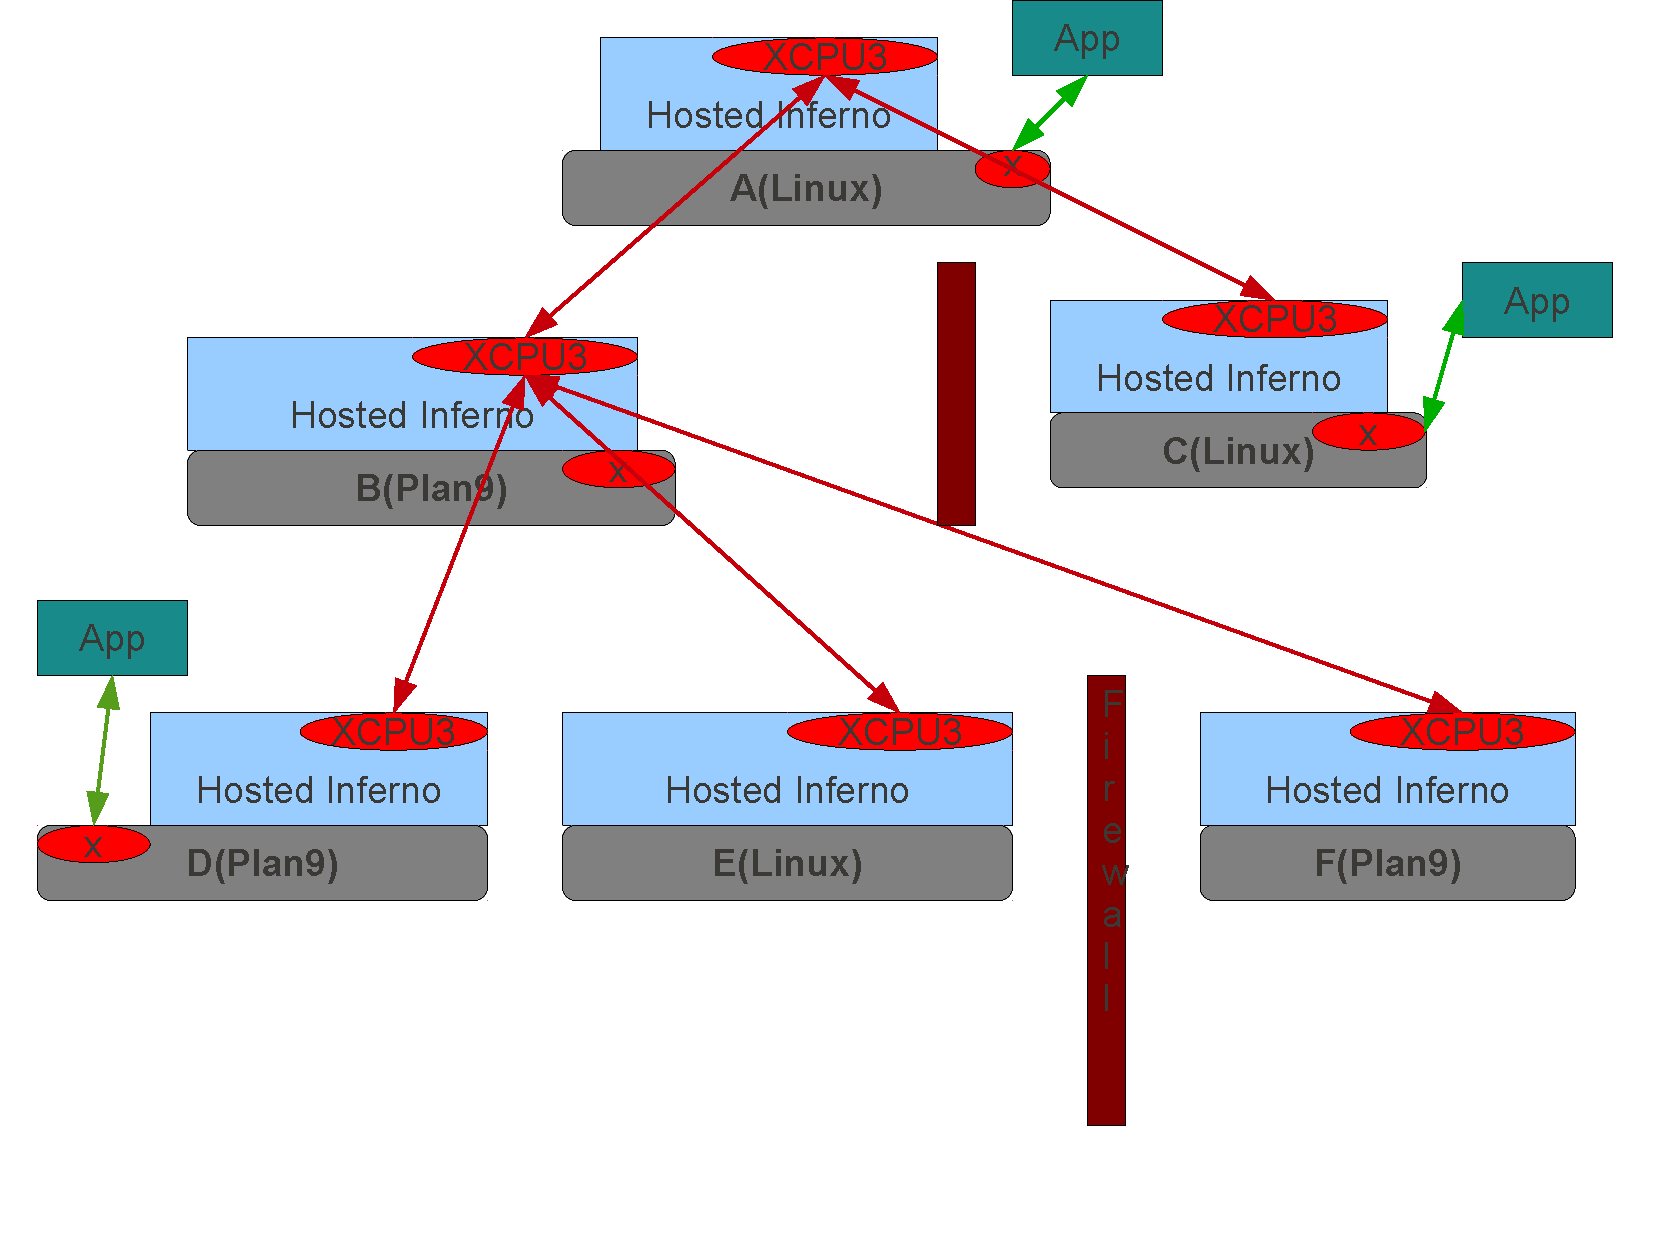
\includegraphics[height=0.4\textheight,width=0.6\textwidth]
		{XCPU3Topo}
    \fi
    \caption{Sample topology of XCPU3}
    \label{fig:XCPU3Topo}
  \end{center}
\end{figure}

This example shows a hierarchical topology with three levels and with a couple
of nodes behind a firewall.  As ducts between XCPU3 filesystem are two-way, it
allows node behind the firewall to participate in the larger topology as long as they
at least have one link with any other node.  In our example, node F can be seen
and accessed by any other node via node B.  The interface for such access is 
explained in \textit{Filesystem interface} section. This way, central services 
play's key role in overcoming the partitioned networks and providing the view of
all resources in network oblivious manner.

\chapter{Filesystem Interface}

This chapter discusses the filesystem interface and how it can be used to access
any node.  We will mainly concentrate on the interfaces for accessing the nodes,
local resources, sessions and sub-sessions.

\section{Interface for remote nodes}
XCPU3 follows certain conventions which allows every node to easily 
interpret the filesystem view of the other nodes.  This section describes 
the XCPU3 interface and the conventions for accessing the remote nodes.

\begin{figure}[h]
  \begin{center}
    \leavevmode
    \ifpdf
      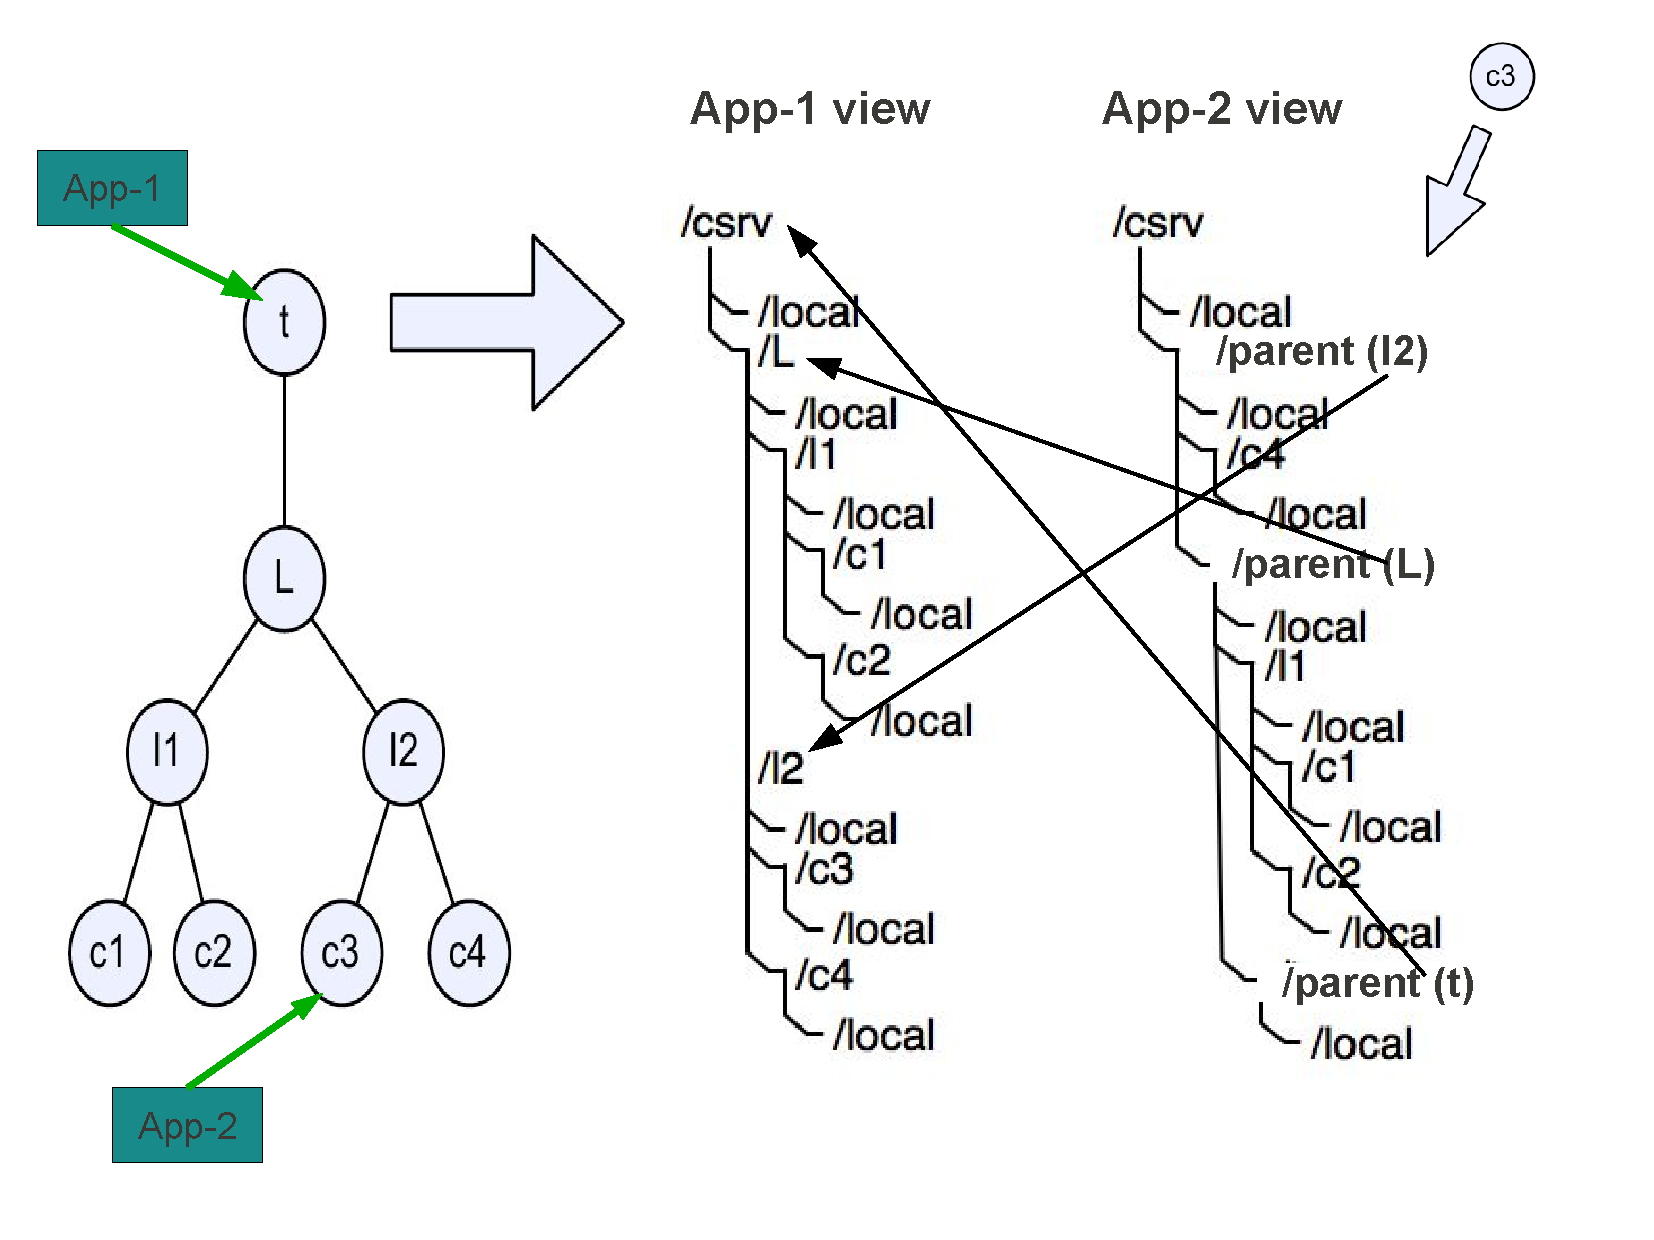
\includegraphics[height=0.3\textheight,width=0.6\textwidth]
		{xcpu3FSTopo}
    \fi
    \caption{Sample filesystem interface for sample the topology in XCPU3}
    \label{fig:xcpu3FSTopo}
  \end{center}
\end{figure}

Figure \ref{fig:xcpu3FSTopo} tries to give a simple overview of how this synthetic
filesystem view is populated based on the underlying topology of the nodes.  The nodes
in the figure are arranged in the simple hierarchical topology.  The XCPU3 filesystem starts with
the \texttt{[/csrv]} directory.  This directory contains the synthetic contents dynamically 
generated by the XCPU3.  The location \texttt{[/csrv/local/]} presents the local resources
whereas \texttt{[/csrv/parent/]} presents the XCPU3 (ie \texttt{[/csrv/]}) filesystem 
of the node which is the parent of this node in the physical topology.  All other directories
in the \texttt{[/csrv/*]} represents the XCPU3 filesystem of the remote nodes which are the children
in the physical topology.  The \textit{App-1 view} is the XCPU3 filesystem view on 
the root node\texttt{[t]}.  You can see that it has two directories in the \texttt{[/csrv/]}
representing the local resources and the remote child L.

The good part of this setup is that every node has to worry about only its children
and the parent, other topology falls in the place automatically. In our sample case, 
the node \texttt{[t]} only needs to connect to node \texttt{[L]}.  It can access other nodes
from the filesystem view of the node \texttt{[L]}.  In tern, the node \texttt{[L]} is responsible
for connecting to the node \texttt{[t]} as parent and node \texttt{[l1]}, \texttt{[l2]} as
children.  These connections allow him to access the entire cluster.  This way, 
responsibility of making the connections with other nodes is also \textbf{localized}
leading to better scalability.  The \textit{App-2 view} provides the \texttt{[/csrv/]} 
filesystem view at the leaf node \texttt{[c3]}.  This node \texttt{[c3]} only connects 
to the node \texttt{[l2]} as it's parent and this single connection allows it to view 
the entire cluster.


This particular view of resources is highly dependent on the underlying cluster.
Nodes are directly connected to the neighbors and indirectly connected to other
nodes, hence maintaining the relationship with underlying cluster.  Most
applications may not want a topology based view of underlying resources, but
the uniform view.  For that reason we create an uniform overlay view separately
for every application when they request the reservation.  This overlay view
binds the resources from this underlying hierarchy and hence successfully hides
the complexities created by underlying topology.  As every application receives
its own session directory and all the requested resources are provided within
the same session directory, the application can use all the resources within
its session without worrying about interfering with others or the physical
location of resources.  As each application lives in it's own session, this
design also enables the capability of running multiple applications
simultaneously and independently. 

The XCPU3 infrastructure is designed to work by providing resources in a uniform
way irrespective of the underlying cluster topology.  But there is a class of
applications and users that want to have the view of resources based on the
cluster topology. The view provided by the \texttt{[/csrv/]} caters to the need
of these applications as this view maps the resources to the underlying cluster
topology.


\subsection{Creating a global view}
Even though the filesystem view at different nodes differ from each other, 
all nodes have access to the full topology.  The \texttt{[/csrv/]} filesystem view 
encodes enough information within itself that any nodes can construct the global view 
and figure out their own position within the global view.


Just because every node can construct the global view, does not mean that it must use
this global view for making any decision or performing a typical operation.
The nodes mostly use only the local view for decision making and operations.  This
local view includes the parent node and the children nodes.


The ability to construct a global view is available to the applications running on 
any node which need this information.  This operation is comparatively expensive
as it involves traversing the \texttt{[/csrv/]} filesystem view.  As each directory
in \texttt{[/csrv/]} location except \texttt{[/csrv/local/]} is the XCPU3 filesystem
of a remote node, any node can access the XCPU3 filesystem of other nodes using this
traversal and use this information to build the global view.
The XCPU3 infrastructure provides the interface to generate such global views,
and leaves the decision to use this information at the expense of performance 
to the application developers and users.

\section{Interface for local resources}
This section describes the interface for accessing and managing the local resources 
at any node.  Again this interface is uniform across all the nodes enabling applications
and other nodes to access it in the same way.  All local resources can be accessed
in the location \texttt{[/csrv/local/]}.  Figure \ref{fig:xcpu3Local} shows the typical 
content of this location.


\begin{figure}[h]
  \begin{center}
    \leavevmode
    \ifpdf
      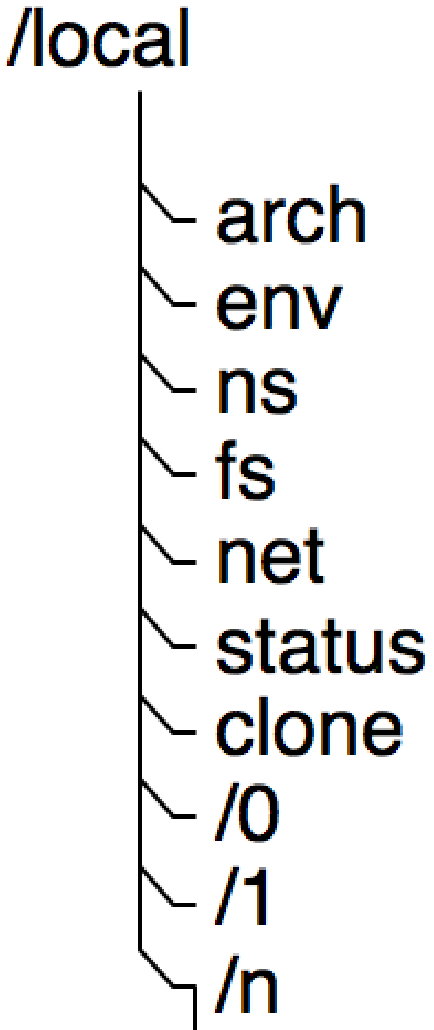
\includegraphics[height=0.4\textheight,width=0.4\textwidth]
		{xcpu3Local.png}
    \fi
    \caption{Sample filesystem interface for local resources in XCPU3}
    \label{fig:xcpu3Local}
  \end{center}
\end{figure}

Each file and directory in the \texttt{[/csrv/local/]} has a specific purpose in accessing
and managing the local resources.
%\begin{enumerate}

\subsection{arch}	\texttt{[/csrv/local/arch]} is a \textit{read-only} file.  A read operation
on this file returns the name of the host operating system and the hardware architecture.
This information is non-destructive and can be read any number of times.
The typical use-case of this file is
\begin{verbatim}
$ cat /csrv/local/arch
Linux 386
$
\end{verbatim}
Typically, this information will be used by the scheduler to satisfy the constraints
imposed by the applications for the underlying operating system and architecture.

\subsection{env} 
\texttt{[/csrv/local/env]} provides the interface for specifying the environmental
variables.  This file can be opened for writing and multiple tuples of \texttt{[Name Value]}
pairs can be written into it.  Following is the example of how this file can be used
\begin{verbatim}
$ echo "PATH /home/example/" > /csrv/local/env
$
\end{verbatim}
The environment variables added this way are the default variables and they will be 
available to all the sessions started on this node.  We do provide another interface
for controlling the environmental variables within a session.  We will discuss that interface in 
more details in the next section.

\subsection{ns} 
\texttt{[/csrv/local/ns]} file provides the interface to assemble the
namespace that will be inherited by any application process created on this node.
\begin{verbatim}
$ echo "mount /exp/root/ /" > /csrv/local/ns
$ echo "bind /some/path /other/path" > /csrv/local/ns
$ 
\end{verbatim}
This is the default namespace and can be overwritten for a particular session using another
interface, allowing more fine-grained control.

\subsection{fs} 
\texttt{[/csrv/local/fs]} location gives the interface to the host filesystem.
This interface allows the applications to access the local filesystem if needed.


\subsection{net} 
\texttt{[/csrv/local/net]} location gives the interface to the host network.
This interface is in the Plan 9 style filesystem which can be used create new network
connections\cite{net}.  The network connections created using this interface will use the local
networking infrastructure.  This is quite useful when the application wants to rely
on the local networking interfaces instead of the abstractions provided by XCPU3.

\subsection{status} 
\texttt{[/csrv/local/status]} is the read-only file providing information about
the available resources at local node and remote nodes.  The information includes
the number of nodes for each combination of an operating system and an architecture.  These
statistics include all the remote nodes which are the descendant of this node. These
descendants are traversed by avoiding the \textit{parent} links.

Every node reads the \texttt{[/csrv/<child-node-name>/local/status]} file of all his children nodes and then
aggregate this information to produce its own status file.  As all the children are XCPU3
nodes themselves, when the parent reads their status file, they repeat the same action
of reading and aggregating the status files of their children.  This way the
process is recursively repeated till it hits the leaf nodes.  These nodes terminate
the recursion by returning the information about themselves. 
Following is an example of the content of status file at a compute node of the Blue Gene
which is a leaf node.
\begin{verbatim}
$ cat /csrv/local/status
1 Plan9 power
$ 
\end{verbatim}

This information is aggregated back till the root node which then returns to the user.
Following is the example of an aggregated information on the Blue Gene computer.
\begin{verbatim}
$ cat /csrv/local/status
1 Linux power
65 Plan9 power
$ 
\end{verbatim}

The above description shows how nodes help each other to perform the operation that needs
the global information.  Unfortunately, these global operations do involve lot of 
communication making them comparatively expensive.  So, hereby we inform the
users about being careful in using these global operations.

We have plans to reduce the cost of such global operations by caching the information 
of previous global operations.  We expect that the global view of the system will
not change very frequently, allowing us to cache this information.  We have not
implemented this yet but we plan to implement such caching in near future.


\subsection{clone} 
\texttt{[/csrv/local/clone]} is a read-write file.  This file is responsible
for creating the sessions which can be used to run the applications.  Whenever this file
is opened, it allocates the session to it.  This session can be a new session with the new
id or a previously used but free session.  The session is identified by the session-id which
is a non-negative number and it is represented as a directory with the session-id value as the name.
The directories \texttt{[/csrv/local/0/]},
\texttt{[/csrv/local/1/]} and \texttt{[/csrv/local/n/]} are the session directories.
Whenever the \texttt{[/csrv/local/clone]} file is opened, a session is allocated to it.
And all subsequent reads on this file will return the session-id of the session
allocated.  Any writes on this opened file will be considered as writes on 
the \texttt{[/csrv/local/<session-ID>/ctl]} file.  If this file is closed and if there
is no other open file within this session directory then this session is released
for future use.

The typical way for using the clone semantic is 
\begin{enumerate}
\item Open clone file in read-write mode.
\item Read the session-id. 
\item Use the files within that session directory for starting and managing the computation.
\item Once your computation is over, close all those files within session.
\item Close the clone file to release the session and the resources allocated. 
\end{enumerate}

\subsection{Sessions} \texttt{[/csrv/local/0/]},
\texttt{[/csrv/local/1/]} and \texttt{[/csrv/local/n/]} are the session directories in
figure \ref{fig:xcpu3Local}. New sessions are created as and when needed and the session-id
value increases monotonically.  Every session directory has its own files with its own
structure.  Next section will discuss the session interface in more details.

\section{Session interface}
This section explains the filesystem interface of the sessions in the XCPU3.
These sessions are important because they are the single unit of execution which can
be entirely controlled by the users.  The figure \ref{fig:xcpu3Local} shows the directory 
structure of a single session.

\begin{figure}[h]
  \begin{center}
    \leavevmode
    \ifpdf
      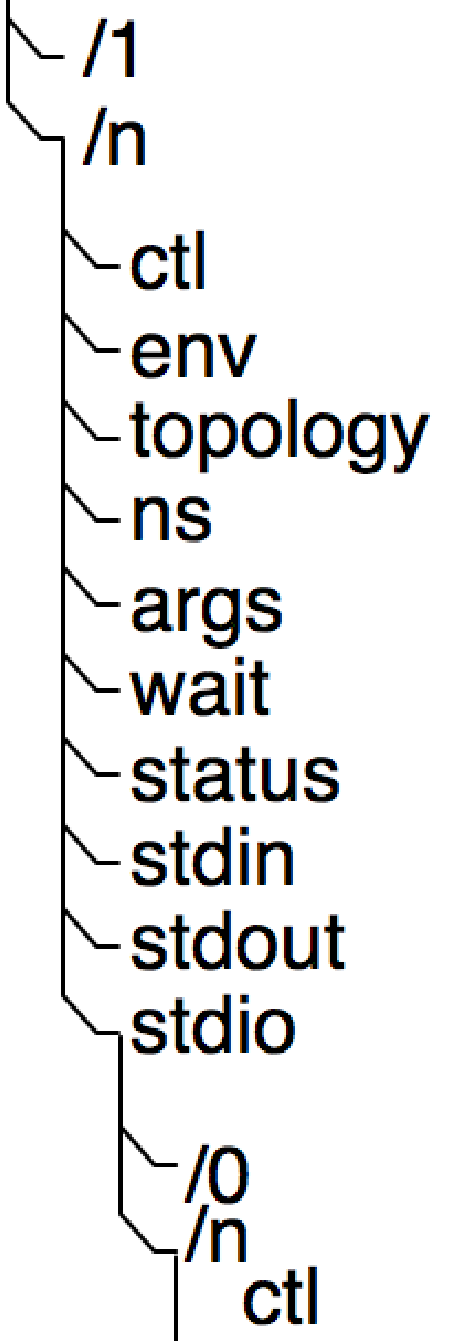
\includegraphics[height=0.44\textheight,width=0.4\textwidth]
		{xcpu3Session.png}
    \fi
    \caption{Sample filesystem interface for sessions in XCPU3}
    \label{fig:xcpu3Local}
  \end{center}
\end{figure}



\subsection{ctl} \texttt{[/csrv/local/<session-ID>/ctl]} is the read-write file which
provides the control over the session.  Just like the clone file, a read operation on this file
will return the session-id.  Write operations on this file are treated as the management commands 
for this session.  These commands can be used to do the reservations of the remote resources,
requesting the execution or the termination of an ongoing execution.

\subsubsection{Reservation request}
The reservation request is one of the most complicated and essential operations in XCPU3, so we are
giving detailed information bellow about how it works.
\begin{verbatim}
$ echo "res 4" > /csrv/local/<session-id>/ctl
$ 
\end{verbatim}
In above request, \textit{res} is the keyword which is followed by the number of resources needed.
Users can also append the type of an OS and an architecture as the constraints if needed, but we are
dropping these advanced options to simplify the explanation.

Satisfying the above request involves the following steps.
\begin{enumerate}
\item Checking the availability of the remote nodes which can be used for the reservations.  
As we have described in the section of the remote node interface, these remote nodes are mounted at 
the \texttt{[/csrv/]} location.
The current implementation selects the children nodes in the round robin fashion.  But we do have 
future plans for making more informed scheduling by accounting for the load on the remote nodes.

Depending on the availability of the children nodes and the number of resources requested, the reservation request
is divided among the selected children, where every selected node is allotted part of the request.

\item   New sessions are created on the selected children nodes by reading their 
\texttt{[/csrv/ <remote-node-name>/local/clone]} file.
In this situation, these newly created sessions are dispersed among the children nodes and are accessible from the filesystem
interface for remote nodes using the path \texttt{[/csrv/<remote-node-name>/ <remote-session-id>/]}.
These resources are not easy to use in the current form as one must have the knowledge of all the remote nodes and 
corresponding session-id for accessing these resources.  We simplify this access by binding these remote
sessions as sub-sessions in the local session directory. In other words we bind 
the \texttt{[/csrv/<remote-node-name>/<remote-session-id>/]} to the \texttt{[/csrv/local/<session-id>/<sub-session-id>/]}.
The sub-session-id's used are monotonically increasing integer numbers starting from the zero.  This way,
all remote resources allocated as part of the reservation request for this session will end up as
the directories within the current session directory.  This arrangement simplifies the interface 
for accessing all the resources associated with one reservation request.

\item The next step is to inform these newly created sub-sessions about their allotted part of the reservation.
This is done by writing the reservation request into their \texttt{[/csrv/local/<session-id>/<sub-session-id>/ctl]}
file.  As the sub-session is an independent session entity, it recursively handles the reservation request by
spreading it among it's children.  This recursion terminates when a node receives the request for reserving zero nodes.
A request for reserving zero nodes is interpreted as the request for local execution.  Once the reservation request
hits this terminating condition, the node reports success to the parent node which in turn reports back success
if all its children nodes also report success.  This reporting leads back to the node which started the 
reservation request.  Once this report reaches back this node, the write operation requesting the reservation
is completed with success.

The current design treats all the errors as fetal.  When any read/write operation fails at any node, it will stop
processing, release any resources that are already alloted and report the error back to the parent.  Once such
error reaches the parent, it will follow the similar suit and release all resources it has allocated for this request.
This also includes releasing the sub-sessions created on other children nodes.  The error is reported to its
parent when all resources are released.  This way error propagates back till the user/application as error in
the write request.

\end{enumerate}

You can observe that above small method creates a tree of sub-sessions where each sub-session maps to the session on
the child node and not necessarily a session where execution will happen.  The leaf sessions are 
responsible for performing the actual execution.  The number of children that
any non-leaf node can have is limited by number of direct neighbors it is
having.  This is because every node can create only one sub-session on remote
nodes, hence limiting the number of sub-sessions to number of neighboring nodes.
The side-effect of this design is that the structure of sub-session's tree
is highly dependent on how nodes are connected with each other at underlying
cluster topology.

Applications which need to control all the computations individually need to
know the topology for locating the leaf sessions.  This is undesirable as we do
not want to expose the applications to underlying network topology.

We could have easily created a flat hierarchy of sub-sessions where each sub-session represents a leaf session 
where the actual execution will happen.  This design ensures that sessions responsible for the actual 
computation are at the same level, hence can be easily accessed.  But we believe that this representation 
of sessions will not scale well for very large numbers of nodes.  The problem in this representation is that it will 
lead to a session directory with a large number of sub-session directories
making it slow for traversing and other directory level operations.  The work
done in the tree spawn algorithm of XCPU shows that hierarchical trees scale
better than a flat hierarchy.  Also, the flat hierarchy with a single root
design puts all the responsibility of workload distribution on the single root
node.  Such uneven distribution of the load makes this approach non-scalable.

On the other hand, the hierarchical tree of the sub-sessions adds more layers
in-between leading to the better distribution of the leaf sessions.  Each
non-leaf session is responsible for a relatively small number of children
nodes. Another advantage with the hierarchical tree design is that each non-leaf
session helps in the workload distribution.
Even though the hierarchical tree design complicates the process of locating the
leaf nodes, the benefits
provided on the scalability front out-weigh this limitation.  We also try to
overcome this limitation
by providing the \texttt{[topology]} file to simplify the problem of locating 
the leaf nodes of the session.


Each node has to initiate this recursive reservation process on each selected
child node by performing a write operation. If these nodes do these reservations
sequentially on each child, the total time taken for the entire reservation
to complete will be proportional to the total number of nodes involved, and
hence not scalable for large reservation requests.


Our implementation does these recursive reservations in parallel for each child
node.  Separate Inferno kernel threads are used to perform the writes on the
children nodes.  This parallel reservation is proportional to the height of the
hierarchical sub-session tree instead of the number of nodes in the tree. This
way, even though we use multiple recursions for making the reservation, we do
them in parallel and save significant amount of time in the process.


A reservation request is the first thing that a user needs to do with the
session.  Once the reservation is done, the session is ready for execution. 
But in case the execution request is submitted without the reservation request,
the XCPU3 will still honor that request by treating it as a local execution
request.

\subsubsection{Execution request}
Execution requests are made by writing them in the \texttt{[ctl]} file. 
Following is a sample execution request.
\begin{verbatim}
$ echo "exec date" > /csrv/local/<session-id>/ctl
$ 
\end{verbatim}
The above example is the request for the execution of the \texttt{date} command.
Here \textit{exec} is the keyword which marks this write operation as
an execution request. If this session is the leaf session (without any
sub-sessions) then this request is executed locally by a specially created
process with the proper namespace and environment variables.


If this session has sub-sessions, then this execution request is distributed
to all the sub-sessions by writing it to their \texttt{[ctl]} file.  This way,
the execution request is propagated till it reaches the leaf sessions where it
is actually executed. All non-leaf sessions act as the workload distribution
points leading to a scalable distribution. Figure \ref{fig:distributionCTL}
shows how the write operations on the \texttt{[ctl]} are distributed in the
session tree.

\begin{figure}[h]
  \begin{center}
    \leavevmode
    \ifpdf
      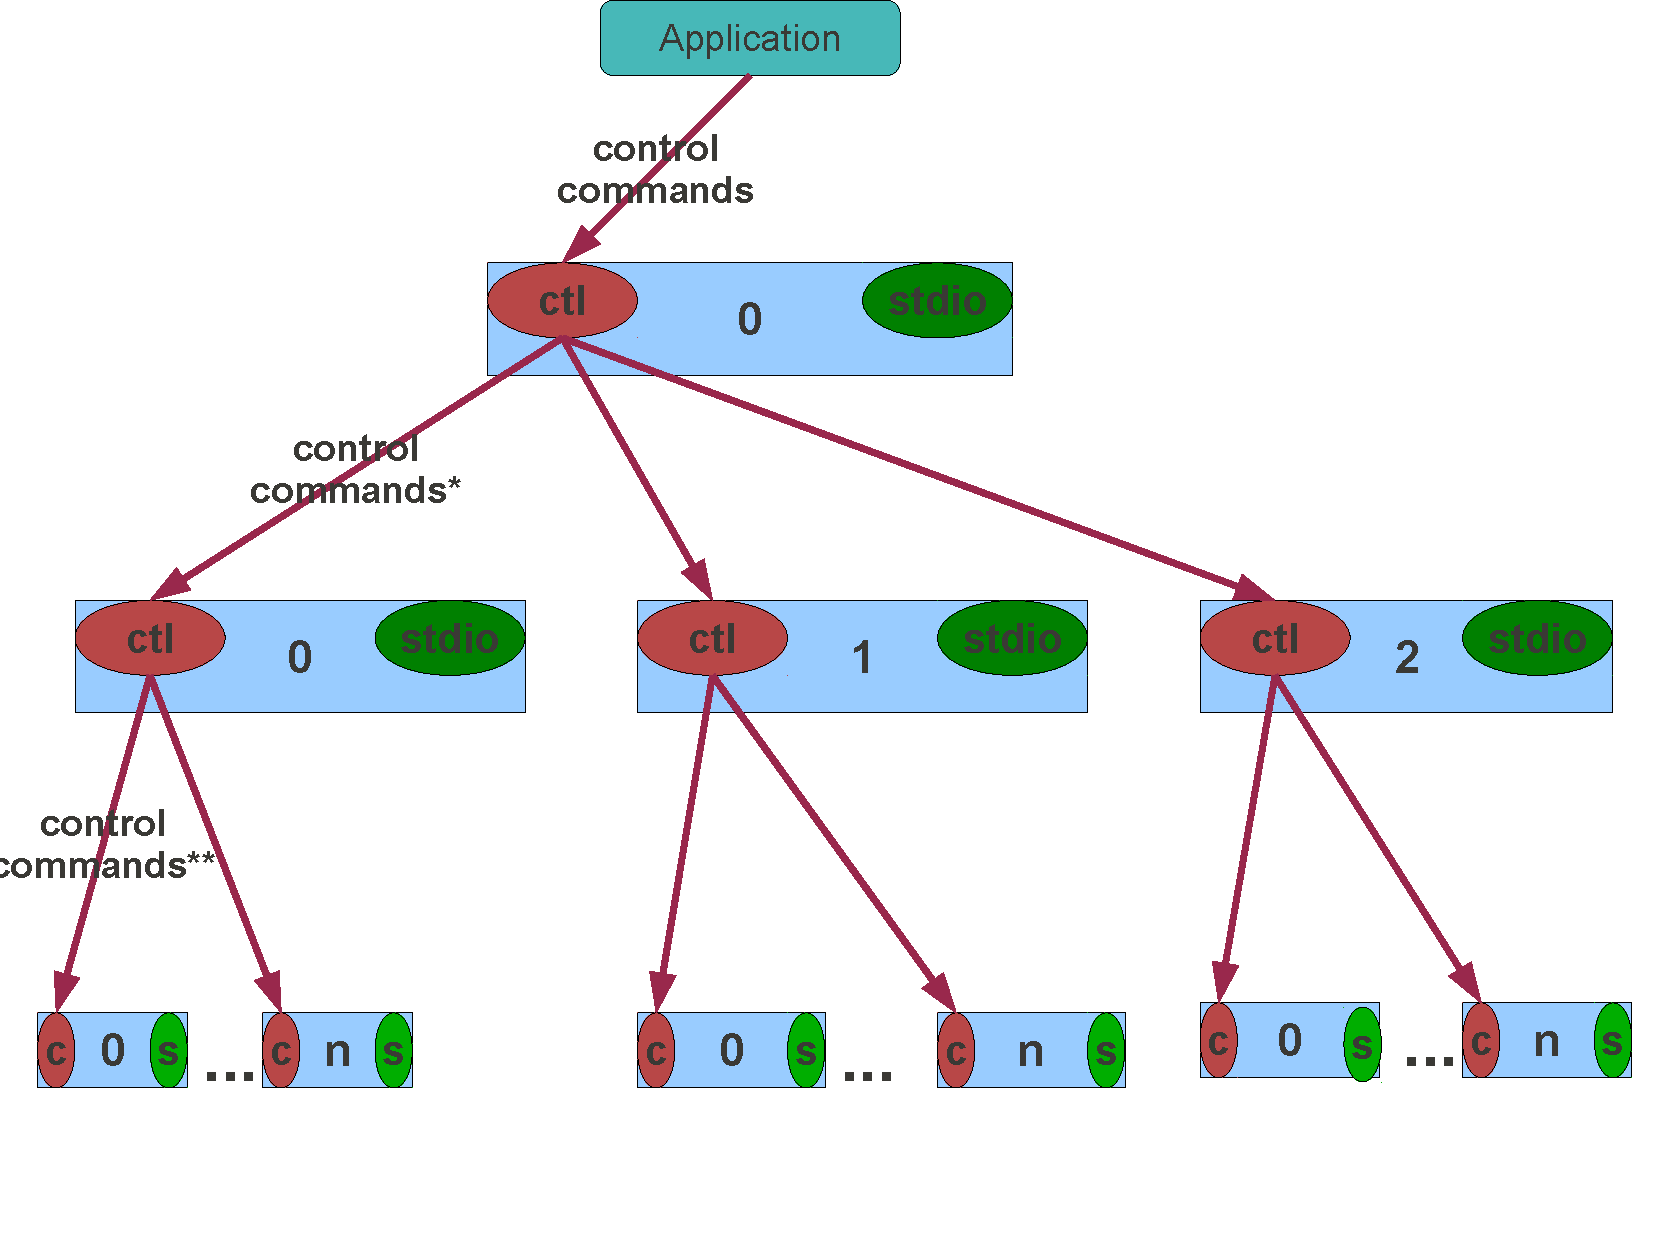
\includegraphics[height=0.44\textheight,width=0.7\textwidth]
		{distributionCTL}
    \fi
    \caption{Distribution of ctl commands}
    \label{fig:distributionCTL}
  \end{center}
\end{figure}

Just like reservation requests, execution requests are also blocking.  So we use
the Inferno kernel threads to handle them in parallel for performance reasons.

\subsubsection{Execution termination}
Any ongoing executions can be terminated by writing the \textit{kill} keyword
into the \texttt{[ctl]} file.  Following is a sample of its usage.
\begin{verbatim}
$ echo "kill" > /csrv/local/<session-id>/ctl
$ 
\end{verbatim}

Just like the \textit{exec} request, this request is recursively propagated till 
the leaf sessions where it is actually performed by killing the process with the help of 
the host operating system.


\subsection{stdio}
\texttt{[/csrv/local/<session-ID>/stdio]} is the read-write file which works as both
standard input and standard output for the application depending on in which mode
the file is opened.  The historical reason behind merging the standard input and the standard 
output into one file is to maintain the compatibility with XCPU and XCPU2.  This
file is responsible for providing the input to the application and returning the
output that application has generated.


\subsubsection{Distributing input}
The input can be provided to the application by writing it into the \texttt{[stdio]} file.
If this session is responsible for the execution, and does not have any sub-sessions then
the input written into this file is directly provided to the standard input descriptor
of the process executing the requested application.

When the session is the aggregation point of the sub-sessions then writing data into the \texttt{[stdio]}
leads to the distribution of that data to all the sub-sessions.  This distribution is done by
writing the received data into the \texttt{[stdio]} file of all the sub-sessions.  This
process for distributing the input data is recursively repeated till the leaf sessions
where this data is actually consumed. The diagram \ref{fig:aggregationSTDIN} presents
a simple visual example of how this happens.
\begin{figure}[h]
  \begin{center}
    \leavevmode
    \ifpdf
      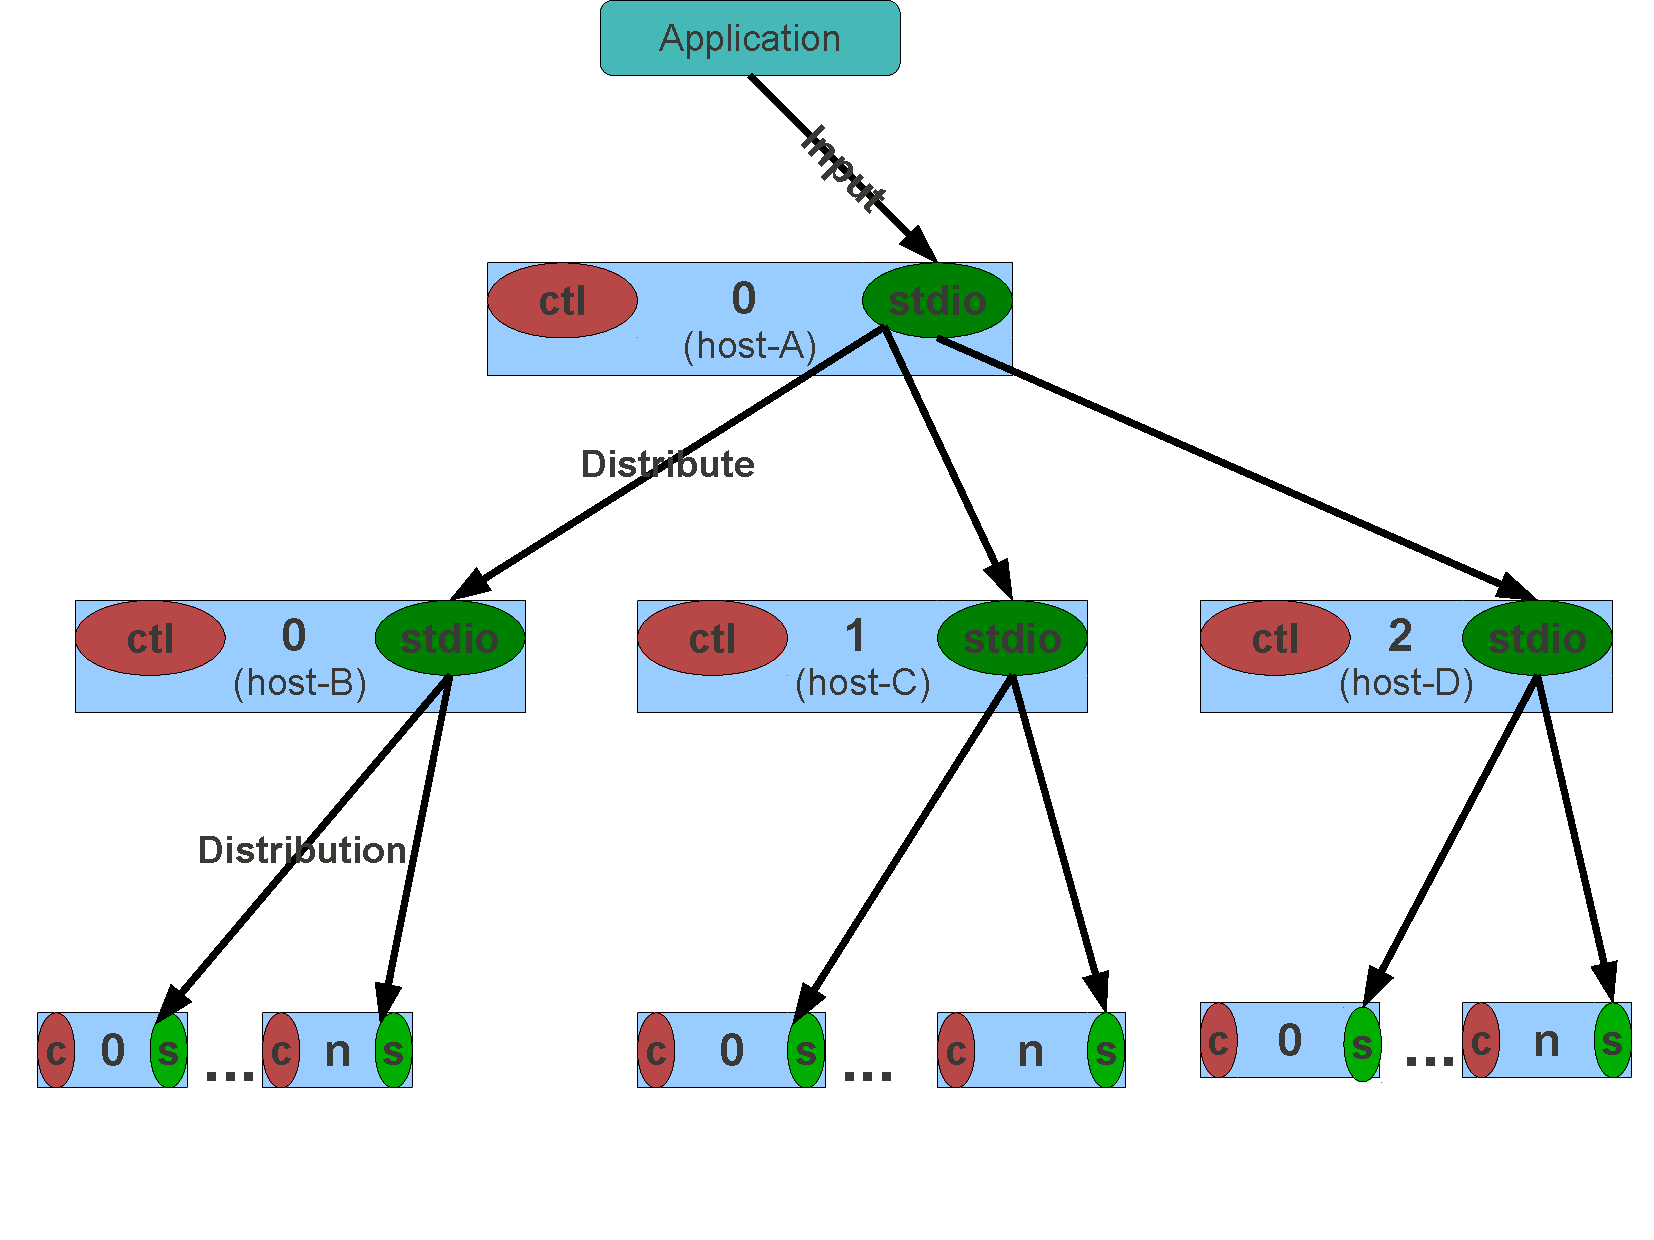
\includegraphics[height=0.44\textheight,width=0.7\textwidth]
		{aggregationSTDIN}
    \fi
    \caption{Distribution of input data}
    \label{fig:aggregationSTDIN}
  \end{center}
\end{figure}

We use separate Inferno kernel threads for distributing the data to each
sub-session.  This way, we avoid the sequential handling of each sub-session
leading to better performance and scalability.  This approach
also ensures that if the write operation on one sub-session is blocked for a
long time,
then it will not delay the delivery of the data to other sub-sessions.

\subsubsection{Aggregating output}
The output of the application can be accessed by reading it from the \texttt{[stdio]} file.
If this session is the leaf session without any sub-sessions, then it signifies that
this session is not the aggregation session but the execution session and the application is 
running in this session.  In such cases, the output is read out from
the standard output descriptor of the process executing the application.  This operation
is performed with the help of the host operating system. 

If it is the aggregation session (i.e. sub-sessions are present),
then the read operation is forwarded to the sub-session's \texttt{[stdio]} files.  This way
the read operation progresses till it reaches the leaf sessions.  As data is only produced
at the leaf sessions, all the read operations are satisfied by them only. 
Figure \ref{fig:aggregationSTDOUT} presents the visual example of how this
aggregation works.

\begin{figure}[h]
  \begin{center}
    \leavevmode
    \ifpdf
      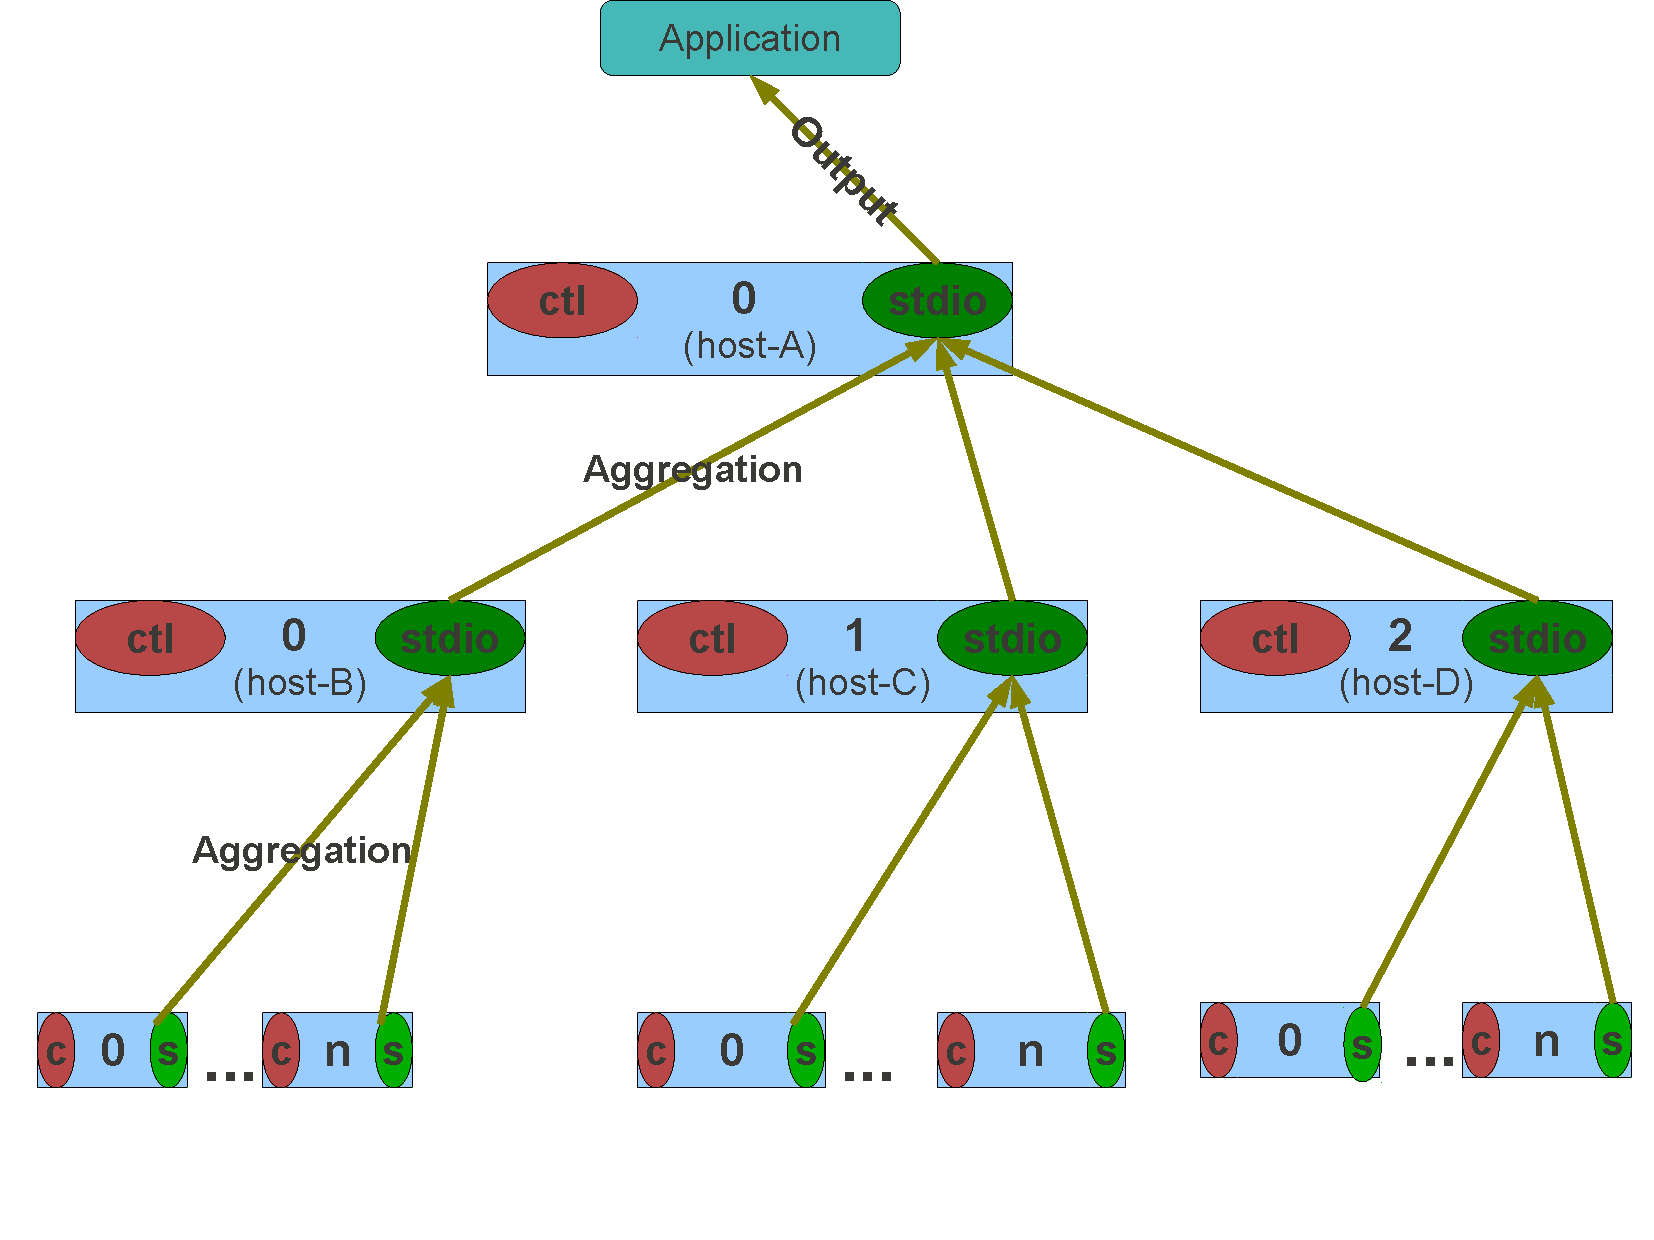
\includegraphics[height=0.44\textheight,width=0.7\textwidth]
		{aggregationSTDOUT}
    \fi
    \caption{Aggregation of input data}
    \label{fig:aggregationSTDOUT}
  \end{center}
\end{figure}

If each node may execute the application with different speed and produce the
output at a different time, then aggregating these outputs becomes complicated. 
We use threads to read the data from each child sub-session so that slower
executions will not block the faster executions.  We use intermediate buffering
at each aggregation sessions.  Data from sub-sessions is read and stored into
these buffers and then any read requests are answered from this buffer.

Output aggregation generates many questions like how does one separate the
output of the two leaf sessions? how does one find out which leaf session
produced which part of the output?  We solve this problem in a related project
(PUSH\cite{push}) which is beyond the scope of this document.


\subsection{wait}
\texttt{[/csrv/local/<session-ID>/wait]} is read only file which provides a
simple way to detect if a requested execution has terminated or not.  This is
done by opening the  \texttt{[wait]} file and reading from it.  This read
operation blocks till the process performing the requested execution terminates.
Whenever the read on this file returns, the user can safely assume that the
requested execution is complete.

Just like the write operations on the session files, this read operation on the
\texttt{[wait]} file is an aggregated read over all the children sub-sessions. 
All the leaf sessions block the read operations on this file within their
session till the process created for the execution is terminated. Once that
process dies, the read is returned.  This way, the \texttt{[wait]} file
facilitates the easy detection of the termination of the computation.

\subsection{env}
\texttt{[/csrv/local/<session-ID>/env]} provides the interface for specifying
the environmental variables.  This provides the same interface as the
\texttt{[/csrv/local/env]} but it affects only the current session instead of
the entire node.  This allows the user to customize each and every session
individually.  If there are sub-sessions, then any write operation on this file
leads to separate and identical write operations on the
\texttt{[/csrv/local/<session-ID>/<sub-session-ID>/env]} files for all the
sub-sessions present in the session.  This way, setting up the environment for
the session leads to setting up the environment for all the reserved nodes.

\subsection{ns}
\texttt{[/csrv/local/<session-ID>/ns]} provides the interface for building the
namespace for the session. This provides the same interface as the
\texttt{[/csrv/local/ns]} but again it affects only the current session instead
of the entire node allowing the user to customize the namespace of each and
every session individually.  Similar to env file, the write operations on the
\texttt{[/csrv/local/<session-ID>/ns]} file trigger separate write operations
on the corresponding \texttt{[ns]} files in every sub-session, leading to
the replication of the namespace on every reserved node.


\subsection{status}
\texttt{[/csrv/local/<session-ID>/status]} is a read only file which reports
the status of the each execution. This information is provided for monitoring
purposes to the users.  Again, this information is generated at the leaf
sessions with the help of the host operating system and is reported back to the
requesting parents.  These parents aggregate all the information and propagate
it back to their parent, till it reaches the starting node.

\subsection{topology}
As we have discussed in the ctl file section, the
\texttt{[/csrv/local/<session-ID>/topology]} file is supposed to provide the
information about the exact location of the sessions which are doing the
executions. The \texttt{[topology]} file does this by providing the relative
path from the current session to every leaf sub-session which is responsible for
the execution.  Any application which needs this information can read and parse
the \texttt{[topology]} file to get this information.

As no single node has global knowledge, the content of the topology file is
generated by recursively merging knowledge of all the nodes participating in
reservation.

\subsection{sub-sessions}
Figure \ref{fig:xcpu3Local} shows an example of sub-sessions \texttt{[0]} and
\texttt{[n]}. These sub-sessions automatically appear in the filesystem view
once the reservation request is successfully submitted to the \texttt{[ctl]}
file.  As we have discussed in the reservation section, these sub-sessions are
nothing but the bindings to the actual sessions running somewhere on the remote
child node. These sub-session directory bindings are temporary and will
dis-appear as soon as all the files in this session directory, including the
\texttt{[clone]} file is closed.  Any operation on the files in session's
directory affects the same file in all the sub-sessions.

The main objective of these aggregation sub-sessions is to achieve better
scalability.  This is done by breaking the large number of requests into the
manageable chunks in hierarchical way.

\section{Examples}
We have been claiming the simplicity of the usability of this infrastructure
through-out the document.  Now is the time to show how easily this system can
be used.  The following examples are designed to show the simplicity of the
system-interface and not to present all available features.  We are giving these
examples of using the bash shell in Linux.  Most parts of these examples are
self explanatory.  We will be giving additional explanations wherever needed.

\subsection{Example of traditional application deployment}
In this example, we show how to run the same application on a large number
of nodes and to collect back their output.  The infrastructure does the workload
distribution and output aggregation automatically on behalf of the application.

We use two terminals for deploying this simple job.  We will use the first
terminal for creating the session, and the other terminal to manage the session
and execution.


We assume that the XCPU3 filesystem is mounted on \texttt{./mpoint/} directory. 
This can be done by using FUSE or 9VFS\cite{v9fseric}.
\begin{verbatim}
$ less ./mpoint/csrv/local/clone
0 
\end{verbatim}
The above shows one of the ways to create a new session.  We use the
\texttt{less} command instead of \texttt{cat} so that the clone file will not be
closed once the End-Of-File (EOF) is detected.  If the clone file is closed
before initiating other actions on this newly created  session, then this
session will be terminated.  We avoid this issue by using the \texttt{less}
command which does not close the file after detecting the EOF. The contents read
from the clone file represent the session-ID.  In our example, the session-ID
is "0".  We will not terminate the \texttt{less} command till we are done with
execution of the application.

Now we use session 0 for performing actual execution.
\begin{verbatim}
$ echo "res 4" > ./mpoint/csrv/local/0/ctl
$ echo "exec date" > ./mpoint/csrv/local/0/ctl
$ cat > ./mpoint/csrv/local/0/stdio
Fri May 7 13:53:58 CDT 2010
Fri May 7 13:53:58 CDT 2010
Fri May 7 13:53:58 CDT 2010
Fri May 7 13:53:58 CDT 2010
$
\end{verbatim}
The first echo command sends the request for reserving 4 remote resources. The
next echo command submits the request for executing the \texttt{date} command.
And the \texttt{cat} command after that returns the aggregated output to the
user.

This example shows all the complexities about finding, connecting and using
the remote resources is hidden behind the filesystem interface.  The reservation
request is responsible for locating the resources, and the execution request is
responsible for initiating the execution of the \texttt{date} command.  As the
namespace of the user is shared with all the remote sessions by default,
the same \texttt{date} command from the client namespace is used for all the
executions.  Reading the stdio file will return the output aggregated from all
the sub-sessions involved in the execution.


Once the execution is over, the \texttt{less} program in the first terminal can
be terminated.  This will close the clone file leading to reclamation of the
used resources and closing of the session.

This approach can be used in the \textit{trivially parallelizable applications}
where the same application is deployed on all the nodes but with different
inputs.  The output from all the nodes involved is merged back to generate the
final result.

This approach can be also used in \textit{high performance computing(HPC)
application} deployments where the underlying infrastructure is only responsible
for deploying the same application on all the nodes, and then the application
itself co-ordinates the workload distribution by communicating with each other.


\subsection{Example of dataflow application deployment}
As we have discussed in the \textit{introduction} chapter, dataflow applications
need flexibility. We will show here, how this flexibility is provided by XCPU3. 
In this mode of operation, the role of XCPU3 is limited to the reservation. 
An application is given the capability of doing the workload distribution and
aggregation with the help of the filesystem interfaces provided by the XCPU3.
Instead of interacting with the aggregation points, these dataflow applications
can interact directly with the sessions responsible for the actual execution
using the filesystem hierarchy of that session.

In this example, we will try to create a small pipeline of two commands
\texttt{date | wc}.  But we will create this pipeline across multiple nodes. 
The objective of this example is to show how the underlying complexities are
hidden from the application.

\begin{verbatim}
$ less ./mpoint/csrv/local/clone
0 
\end{verbatim}
The above command creates the session in the same way we described in the
previous example.  The following commands will create the desired pipeline.

\begin{verbatim}
$ echo "res 2" > ./mpoint/csrv/local/0/ctl
$ echo "exec date" > ./mpoint/csrv/local/0/0/ctl
$ echo "exec wc" > ./mpoint/csrv/local/0/1/ctl
$ echo "xsplice 0 1" > ./mpoint/csrv/local/0/ctl
$ cat ./mpoint/csrv/local/0/1/stdio
1 6 29
$
\end{verbatim}

Now, we want to create a pipeline of two commands, so we have reserved two
remote resources using the first command.  Now, instead of the aggregation, the
following commands directly traverse the session directory structure one level
deeper and request the individual executions on each of the nodes.  The first
command \texttt{[exec date]} is sent to 0'th sub-session and the second command
\texttt{[exec wc]} is sent to the 1st sub-session.  The \texttt{[xsplice 0 1]}
request tells the parent session to redirect the output of the 0'th session to
the input of the 1st session.  The \textbf{xsplice} command can be seen as a
pipe operator of the shell script for redirecting the output of one command to
the input of other command.  The only difference is that the xsplice operator
connects the two sessions instead of connecting two commands.

The above example is equivalent of executing \texttt{date | wc} on the shell,
but with the difference that both commands are executed on a different remote
machines while sharing the same namespace.

We do need few more mechanisms for easily mapping the DAG of dataflow
applications onto XCPU3 infrastructure.  Most notable mechanisms are the
\textbf{inflow} and the \textbf{outflow} operators.  The inflow operator can be
seen as the mechanism for distributing the output generated by one compute
vertex to the input of multiple compute vertices.  The outflow operator
aggregates the output of multiple compute nodes and redirects it as input to one
compute node.

We do not implement these inflow and outflow operators in the XCPU3
infrastructure directly but we have left this responsibility to userspace
applications like the \textbf{PUSH shell}\cite{PODC:Push}. This shell is
designed to take a dataflow application, convert it into the DAG, map it
onto the remote resources reserved by the XCPU3 and orchestrate the flow of the
data between all the compute vertices (i.e. compute sessions). The XCPU3 is the
infrastructure where operators needed for dataflow applications like the inflow
and the outflow can be easily implemented.


%\end{enumerate}
% ------------------------------------------------------------------------

%%% Local Variables: 
%%% mode: latex
%%% TeX-master: "../thesis"
%%% End: 
